\documentclass[12pt]{article}
\usepackage{graphicx}
\usepackage{times}
\usepackage{cite}
\usepackage[utf8]{inputenc}
\usepackage{subfig}
\usepackage{caption}
%this is a comment
\title{The Memo}
\author{Jesse Chick\\
\and Benjamin Martin\\
\and Keenan Johnson\\
\and Nickoli Londura\\
\and Jiaji Sun}




\begin{document}
\maketitle
\tableofcontents

\section{Contributors and ONIDs}
\begin{itemize}
	\item Jesse Chick $\sim$ chickj
	\item Benjamin Martin $\sim$ martinb3
	\item Keenan Johnson $\sim$ johnsoke
	\item Nickoli Londura $\sim$ londuran
	\item Jiaji Sun $\sim$ sunji
\end{itemize}

\section{User Interface Prototypes}

	\subsection{Tutorials Page}
	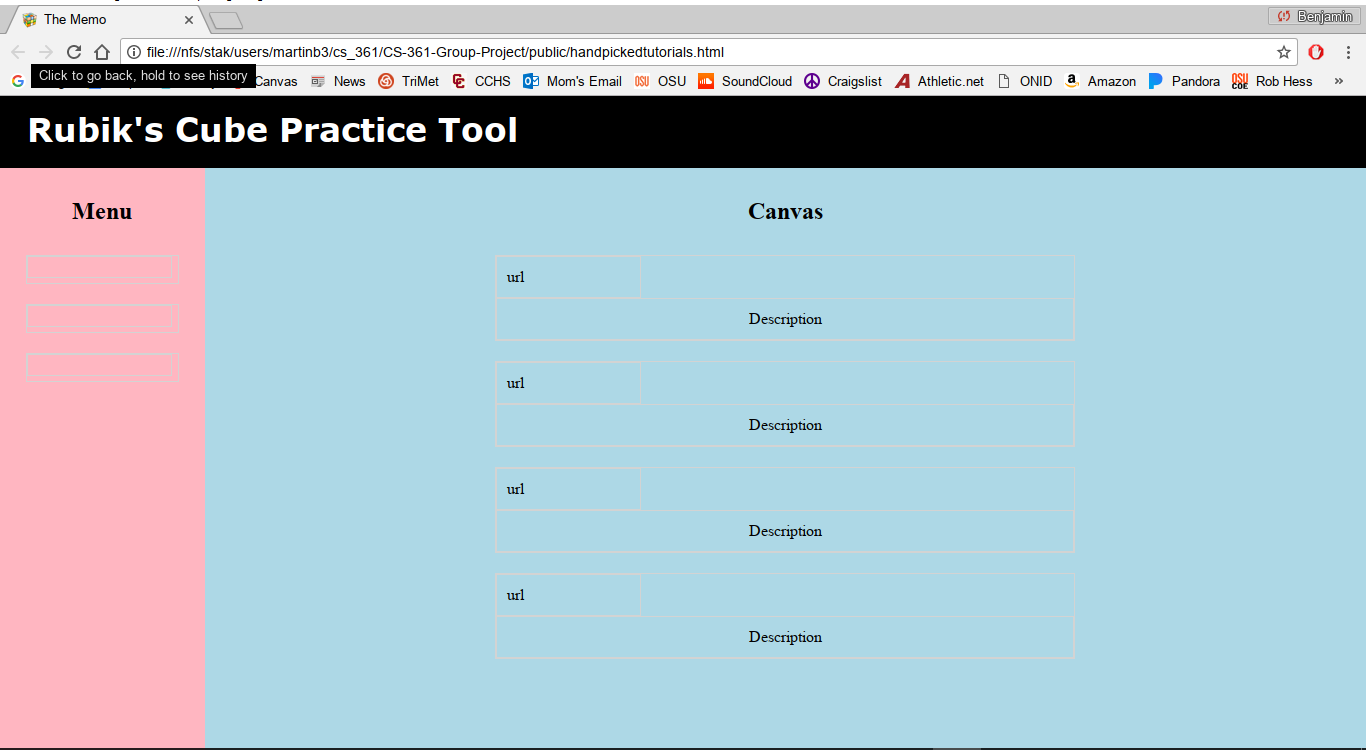
\includegraphics[width = \textwidth]{tutorial.PNG}
	\subsection{Rubik's Cube practice page}
	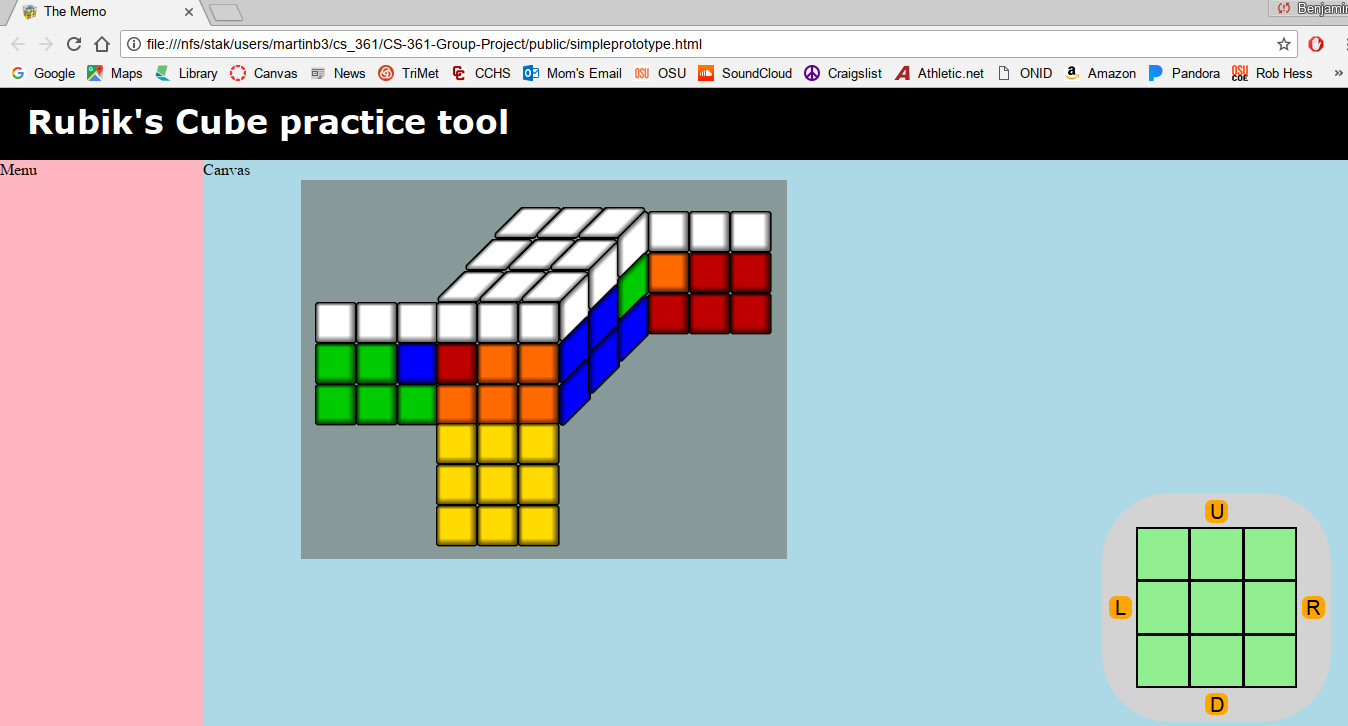
\includegraphics[width = \textwidth]{cubepage.PNG}
	\subsection{Letter memorization page}
	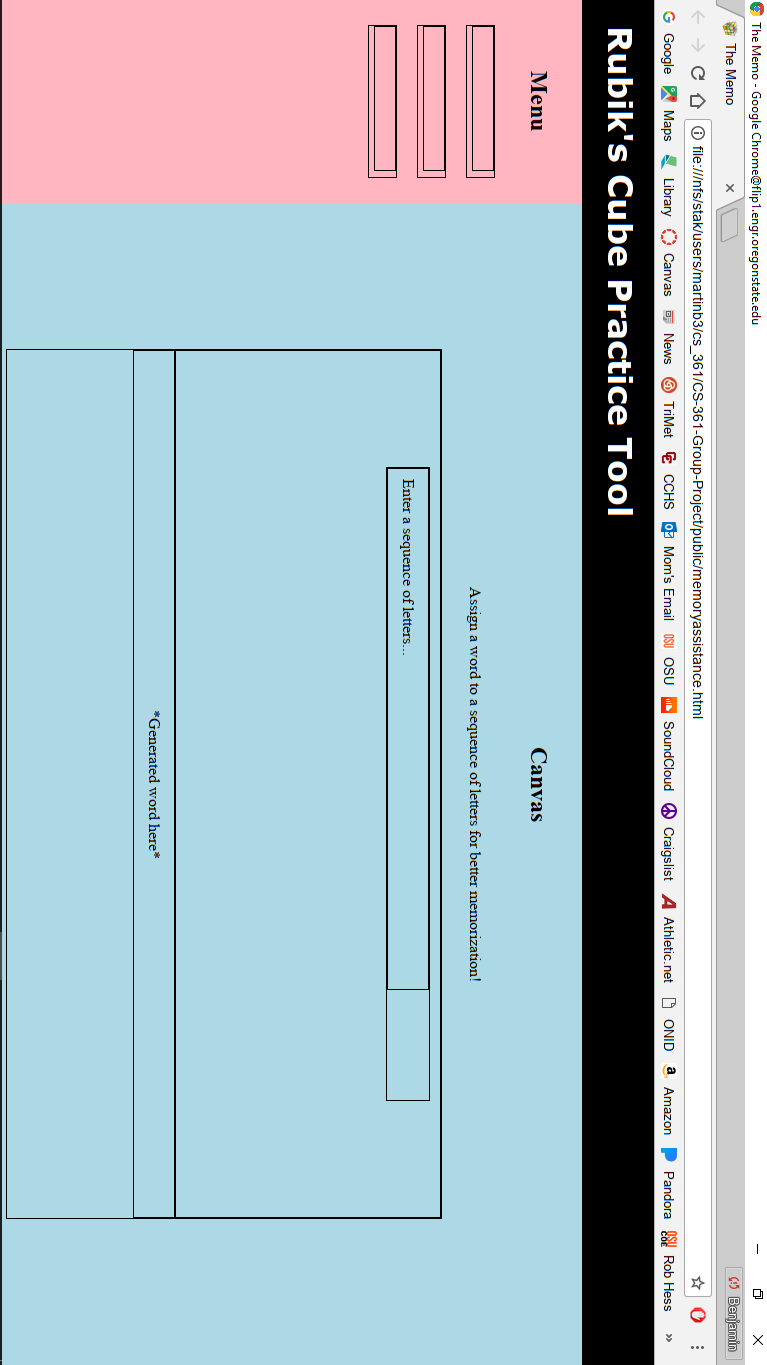
\includegraphics[width = \textwidth]{lettermem.PNG}


\section{Class Diagrams}

	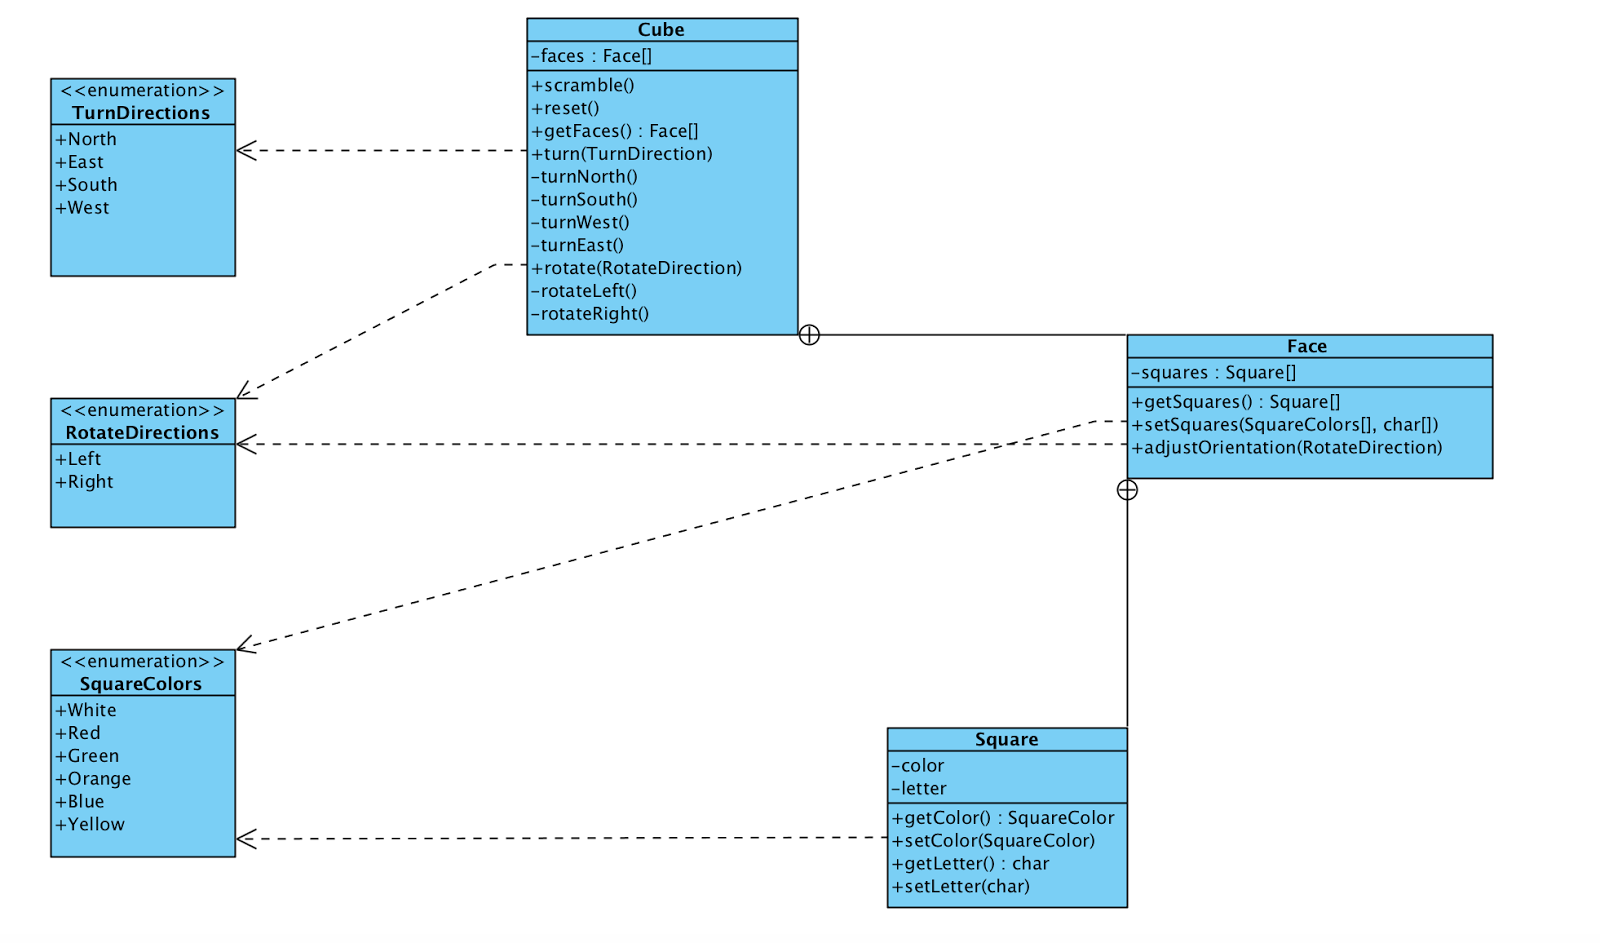
\includegraphics[width = \textwidth]{diagram.PNG}
	

\section{Sequence Diagrams}

\section{Meeting Report}

\par
On this week we have met 4 times on campus. Including three times in library and one meeting after class. \\

\par
On our first meeting on Wednesday. We met everyone in the library. we separate our second phase of the project to every group member. Jesse Chick is working on Class Diagrams. Benjamin Martin is working on Sequence Diagrams. Jiaji Sun is working on meeting report. Nickoli Londura is working on part of User Interface Prototypes. Keenan Johnson is working on scramble code and solution generation. On this meeting, we have drawn basic prototype of our project, and basic design each functions for every function. At the beginning, we drew a basic section of the prototype on paper, then rough design each functions for every function. Then we modify the design multiple times. Finally, we settle down the first version of the project. On this meeting, we find a new feature about our project is we implement one that generates easy to memorize words for given letter pairs. Example: given the letter pair CT would output an easy to memorize word such as ‘cat’. At the end of this meeting, we set up next meeting time. \\

\par
On our second meeting, we met after class. Everyone describes new idea of each other. We are thinking about the new design of our project, and everyone has talked about their new idea of our project. After we discussed our new design. We decide to keep discussed our project design at next meeting. Then we set next meeting time. \\

\par
On our third meeting, we met everyone in the library. we decide change design for our project. Jesse start modifies class diagrams into a new design. Benjamin also modifies his sequence diagrams into a new design. Nickoli starts working on the first version of prototypes of the project. Keenan is working on try to making code work well and smoothly. After we changed our design, the new version of our project design is come out. \\

\par
On our fourth meeting, we still met in the library. We have discussed our last version of project design and final version of prototypes. Jesse keeps working on class diagrams. Benjamin keeps working on sequence diagrams. Nickoli keeps working on the prototypes of our project. Keenan compiled every code to make sure it works well. At the end, Jesse and Benjamin finished their diagrams. Nickoli finished the prototypes of the project. Keenan compiled every code, and make every code working well. We have done our parts nicely. \\

\cite{rubtut}

\bibliography{myref}
\bibliographystyle{plain}

\end{document}
